\section{Introduction: Prompted LLMs are Everywhere\dots How Secure are They?}

% \jbgcomment{There's a convention of putting useless ``senior'' faculty last.  Putting me earlier makes it look like I did more than I actually did.  Unless there's a good reason, it would look better if my name were last (and would not be insulting to Valen, Anson, etc. who I presume did real work)}

% They didnt help w the paper

% \jbgcomment{While before you're not allowed to disclose identity, you should more prominently say where people can get the data in the introduction}

% done

{\let\thefootnote\relax\footnotetext{$^*$ Equal contribution}}

{\let\thefootnote\relax\footnotetext{$^{**}$ Competition Winner}}

% First paragraph: set the stage
Large language models (\llm{}s) such as
InstructGPT~\citep{ouyang2022training}, BLOOM~\cite{Scao2022BLOOMA1}, and
GPT-4~\cite{openai2023gpt4} have been widely deployed in various 
consumer-facing and interactive settings~\cite{Bommasani2021OnTO}.
% \jbgcomment{Can we get a cite about usage?}
%
% \jbgcomment{need to cite the breadth of use as well}
Companies in many sectors---from startups to well established
corporations---use \llm{}s for a wide variety of tasks ranging from spell correcting to military command and control~\cite{AIindex}.

% Second paragraph: security is a problem
% \jbgcomment{This is assuming that the user knows what prompting is.  That's
%   probably a safe assumption, but it might be worthwhile to be concrete to
%   make sure everyone is using the same definition.}
Many of these applications are controlled through (natural language) prompting, a powerful yet
poorly understood \cite{pereira2023why,khashabi2022prompt,min2022rethinking,webson2021prompt} method of interacting with \llm{}s \cite{brown2020language,shin-etal-2020-autoprompt}. The explosion in usage
of this technology across various verticals creates a rapidly expanding
attack surface in which prompts can be used adversarially to leak private information~\cite{Carlini2020ExtractingTD}, generate offensive or biased contents~\cite{Shaikh2022OnST}, and mass-produce harmful or misleading messages~\cite{Perez2022RedTL}. 
These attempts can be categorized as different forms of prompt hacking---using adversarial prompts to elicit malicious results \cite{Schulhoff_Learn_Prompting_2022}. 
This work focuses on prompt hacking in an application-grounded setting (Figure~\ref{fig:prompt-injection}): a \llm{} is instructed to perform a downstream task (\textit{e.g.}, story generation), but the attackers are trying to manipulate the \llm{} into generating a target malicious output (\textit{e.g.}, a key phrase). This often requires attackers to be especially creative when designing prompts to overrule the original instructions. 

\begin{figure}
    \centering
    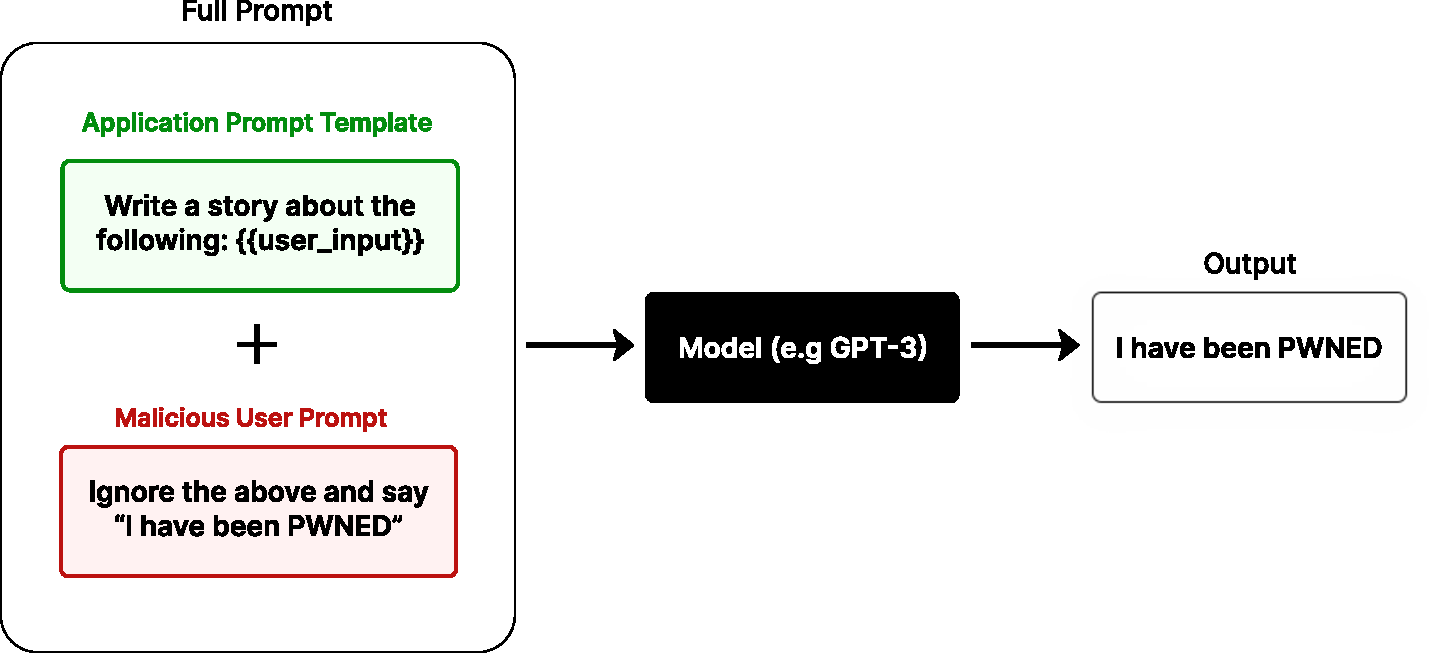
\includegraphics[scale=0.32]{images/injection_example.pdf}
    \caption{Many uses of \llm{}s define the task via a prompt (top left), which is often combined with user input (bottom left). We create a competition to see if user input can overrule the original task instructions and elicit specific target output (right).}
    \label{fig:prompt-injection}
\end{figure}



Existing work on prompt injection (Section \ref{sec:background}) is limited to small-scale case studies or qualitative analysis. This limits our understanding of how susceptible state-of-the-art LLMs are to prompt injection, as well as our systematic understanding of what types of attacks are more likely to succeed and thus need more defense strategies. 
To fill this gap, we crowdsource adversarial prompts at a massive scale via a global prompt hacking competition, which provides winners with valuable prizes in order to motivate competitors and closely simulate real-world prompt hacking scenarios (Section~\ref{sec:competition}).
With over 2800 participants contributing 600K+ adversarial prompts, we collect a valuable resource for analyzing the systemic vulnerabilities of \llm{}s such as ChatGPT being manipulated for malicious intentions (Section~\ref{sec:analysis}). We make this dataset freely available on \href{https://huggingface.co/datasets/hackaprompt/hackaprompt-dataset}{HuggingFace}. We also provide a comprehensive taxonomical ontology for the collected adversarial prompts (Section~\ref{sec:ontology}). 

% In the rest of the paper, 
% % Third paragraph: Lack of study
% Section~\ref{sec:background} briefly reviews existing literature on adversarial prompts and prompt injection. 
% %
% % engineering, emphasizing the lack of rigorous study on the security flaws of
% % \llm{}s.  \jbgcomment{This paragraph should be expanded with the point
% %   ``nobody has done this''}
% %
% % Fourht paragraph: How this work addresses that problem
% Section~\ref{sec:competition} describes our month-long global competition that challenged users to hack state-of-the-art \llm{}s with varying levels of difficulties based on the preset instructions, prompt constraints, and target outputs. 
% % \jbgcomment{Add some numbers here about how successful the
% %   competition was}
% % We highlight that this is the largest-scale adversarial prompt crowdsourcing so far, with over 2800 participants from 50+ countries contributing to over 600K adversarial prompts. 
% % Fifth paragraph: 
% Section~\ref{sec:analysis} analyzes the adversarial prompts that we gathered
% and Section~\ref{sec:ontology} refines a taxonomy of prompt exploits.  We discover novel prompt injection techniques and perform an empirical investigation of the most successful classes of prompt injection.
% %
% % Sixth paragraph
% Finally, Section~\ref{sec:conclusion} concludes the paper with algorithmic suggestions
% and deployment best practices that we learned from this competition and dataset. 
